\begin{center}
  \scalebox{1.0}{
    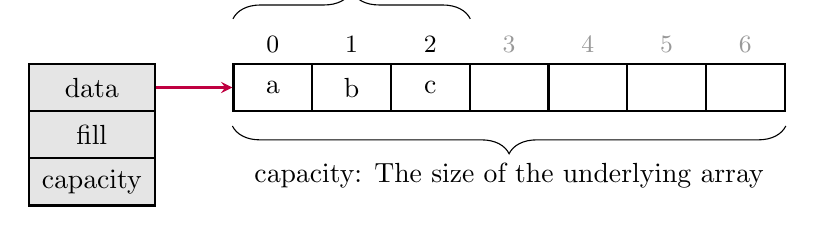
\begin{tikzpicture}[]
      \coordinate (origo) at (0mm,-6cm);
      
      \tikzstyle{cell} = [
        rectangle,
        draw=black,
        thick,
        anchor=west,
        minimum width=10mm,
        minimum height=6mm,
      ]
      \tikzstyle{celllabel} = [
        draw=none,
        anchor=south,
        align=center,
        minimum width=10mm,
      ]
      
      \tikzstyle{arrow} = [overlay, thick,->,>=stealth, draw=purple]
      
      % object
      \node[cell,fill=black!10,minimum width=16mm] (celldata) at ([xshift=0mm] origo) {data};
      \node[cell,fill=black!10,minimum width=16mm] (cellfill) at ([xshift=0mm,yshift=-6mm] origo) {fill};
      \node[cell,fill=black!10,minimum width=16mm] (cellcapacity) at ([xshift=0mm,yshift=-12mm] origo) {capacity};
      
      % elements
      \node[cell] (cell1) at ([xshift=26mm] origo) {a};
      \node[cell] (cell2) at ([xshift=36mm] origo) {b};
      \node[cell] (cell3) at ([xshift=46mm] origo) {c};
      \node[cell] (cell4) at ([xshift=56mm] origo) {};
      \node[cell] (cell5) at ([xshift=66mm] origo) {};
      \node[cell] (cell6) at ([xshift=76mm] origo) {};
      \node[cell] (cell7) at ([xshift=86mm] origo) {};
      \node[celllabel] (cell1label) at ([xshift=0mm] cell1.north) {\small 0};
      \node[celllabel] (cell2label) at ([xshift=0mm] cell2.north) {\small 1};
      \node[celllabel] (cell3label) at ([xshift=0mm] cell3.north) {\small 2};
      \node[celllabel,text=black!40] (cell4label) at ([xshift=0mm] cell4.north) {\small 3};
      \node[celllabel,text=black!40] (cell5label) at ([xshift=0mm] cell5.north) {\small 4};
      \node[celllabel,text=black!40] (cell6label) at ([xshift=0mm] cell6.north) {\small 5};
      \node[celllabel,text=black!40] (cell7label) at ([xshift=0mm] cell7.north) {\small 6};
      
      % arrow
      \draw[arrow] (celldata.east) -- (cell1.west);
      
      % braces
      \draw[overlay, decorate,decoration={brace, amplitude=10pt, raise=3pt}] (cell1label.north west) to node[black,midway,above=15pt] {fill: Number of elements (via the  \propertyname{Size}  property)} (cell3label.north east);
      \draw[overlay, decorate,decoration={brace, mirror, amplitude=10pt, raise=5pt}] (cell1.south west) to node[black,midway,below=15pt] {capacity: The size of the underlying array
      } (cell7.south east);
    \end{tikzpicture}
  }
\end{center}
